% Options for packages loaded elsewhere
\PassOptionsToPackage{unicode}{hyperref}
\PassOptionsToPackage{hyphens}{url}
%
\documentclass[
]{article}
\usepackage{lmodern}
\usepackage{amssymb,amsmath}
\usepackage{ifxetex,ifluatex}
\ifnum 0\ifxetex 1\fi\ifluatex 1\fi=0 % if pdftex
  \usepackage[T1]{fontenc}
  \usepackage[utf8]{inputenc}
  \usepackage{textcomp} % provide euro and other symbols
\else % if luatex or xetex
  \usepackage{unicode-math}
  \defaultfontfeatures{Scale=MatchLowercase}
  \defaultfontfeatures[\rmfamily]{Ligatures=TeX,Scale=1}
\fi
% Use upquote if available, for straight quotes in verbatim environments
\IfFileExists{upquote.sty}{\usepackage{upquote}}{}
\IfFileExists{microtype.sty}{% use microtype if available
  \usepackage[]{microtype}
  \UseMicrotypeSet[protrusion]{basicmath} % disable protrusion for tt fonts
}{}
\makeatletter
\@ifundefined{KOMAClassName}{% if non-KOMA class
  \IfFileExists{parskip.sty}{%
    \usepackage{parskip}
  }{% else
    \setlength{\parindent}{0pt}
    \setlength{\parskip}{6pt plus 2pt minus 1pt}}
}{% if KOMA class
  \KOMAoptions{parskip=half}}
\makeatother
\usepackage{xcolor}
\IfFileExists{xurl.sty}{\usepackage{xurl}}{} % add URL line breaks if available
\IfFileExists{bookmark.sty}{\usepackage{bookmark}}{\usepackage{hyperref}}
\hypersetup{
  pdftitle={Sensitivity Analysis},
  hidelinks,
  pdfcreator={LaTeX via pandoc}}
\urlstyle{same} % disable monospaced font for URLs
\usepackage[margin=1in]{geometry}
\usepackage{longtable,booktabs}
% Correct order of tables after \paragraph or \subparagraph
\usepackage{etoolbox}
\makeatletter
\patchcmd\longtable{\par}{\if@noskipsec\mbox{}\fi\par}{}{}
\makeatother
% Allow footnotes in longtable head/foot
\IfFileExists{footnotehyper.sty}{\usepackage{footnotehyper}}{\usepackage{footnote}}
\makesavenoteenv{longtable}
\usepackage{graphicx,grffile}
\makeatletter
\def\maxwidth{\ifdim\Gin@nat@width>\linewidth\linewidth\else\Gin@nat@width\fi}
\def\maxheight{\ifdim\Gin@nat@height>\textheight\textheight\else\Gin@nat@height\fi}
\makeatother
% Scale images if necessary, so that they will not overflow the page
% margins by default, and it is still possible to overwrite the defaults
% using explicit options in \includegraphics[width, height, ...]{}
\setkeys{Gin}{width=\maxwidth,height=\maxheight,keepaspectratio}
% Set default figure placement to htbp
\makeatletter
\def\fps@figure{htbp}
\makeatother
\setlength{\emergencystretch}{3em} % prevent overfull lines
\providecommand{\tightlist}{%
  \setlength{\itemsep}{0pt}\setlength{\parskip}{0pt}}
\setcounter{secnumdepth}{-\maxdimen} % remove section numbering

\title{Sensitivity Analysis}
\author{}
\date{\vspace{-2.5em}2 December 2020}

\begin{document}
\maketitle

\hypertarget{data}{%
\subsection{Data}\label{data}}

The information on doors is not really in a usable form, so for this
analysis the door information is recoded into a door state for each
door. The state can be one of ``closed'' ``one-fourth'', ``one-half'',
``three-fourth'', and ``open.'' The recoding for doors is what is used
throughout this analysis.

\hypertarget{number-of-cases}{%
\subsection{Number of Cases}\label{number-of-cases}}

As a first step, we do a preliminary check to see if we have enough
cases. To be meaningful we have to look at one of the output columns;
here we look at the Bedroom 1 Alarm data. Looking at the data it becomes
very quickly apparent that the results for Flaming type fires and
Smoldering type fires are very different. Also, nearly half the cases
have no activation within the simulation time. So the evaluation of
convergence is evaluated separately for flaming type fires and
smoldering type fires. Then the time to activation for cases where
activation occurs is evaluated separately from the percent of cases
where activation occurs. If any of these do not converge, then we do not
have enough cases.

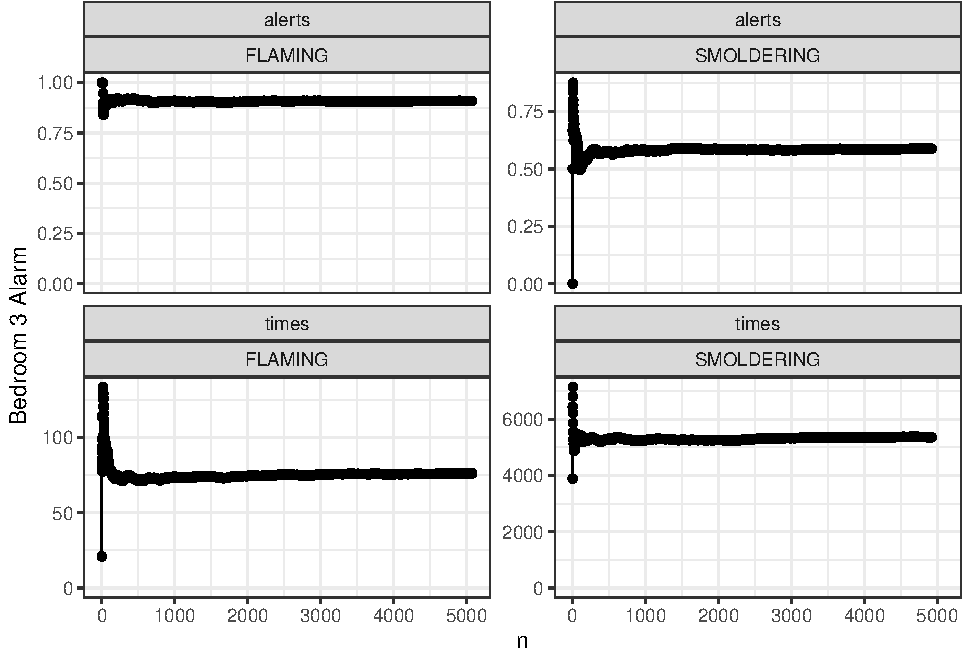
\includegraphics{ex3_files/figure-latex/converg-1.pdf}
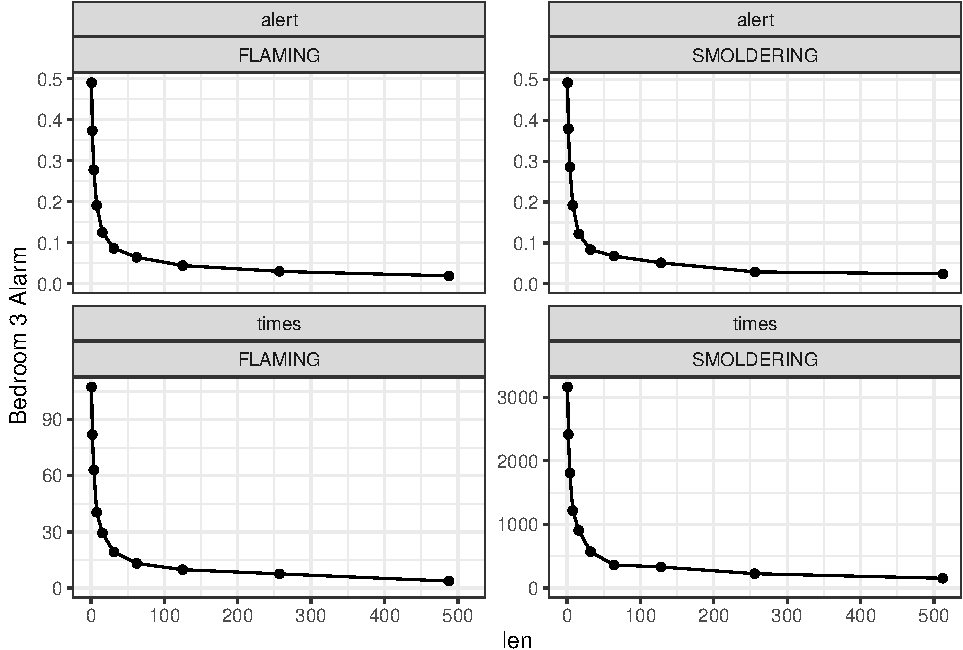
\includegraphics{ex3_files/figure-latex/converg-2.pdf}

The prelinary results, charted above, suggest that we have enough cases.
The averages all appear to have converged, and the standard errors are
small.

\hypertarget{analysis}{%
\subsection{Analysis}\label{analysis}}

The question explored here is the benefit gained by connecting alarms.
The effect of interconnecting alarms is to reduce the amount of time
before people in the house are notified of a fire even though they may
be far away from the location of the fire. In this example, there are
fires in the dining room, kitchen, or living room, and we will assume
that people are in the bedrooms. Further assume the people in the
bedrooms will not hear an alarm unless it is the one in the bedroom. So
the effect of interconnecting alarms is to notify people to a fire when
the alarm in one of the front rooms goes off rather than waiting until
one of the bedroom alarms sounds.

Assume for this example that there is one alarm in the Living Room and
one alarm in Bedroom 1 (which will proxy for all the bedroom alarms).
This example, then, examines the difference in activation times between
the Living Room Alarm and the Bedroom 1 Alarm.

Exploratory analysis of the data is an important part of any analysis.
Here, initial exploration indicated that in a substantial number of
cases one or more of the alarms never activated.

\begin{longtable}[]{@{}lcccc@{}}
\toprule
\endhead
\begin{minipage}[t]{0.17\columnwidth}\raggedright
\strut
\end{minipage} & \begin{minipage}[t]{0.14\columnwidth}\centering
Bedroom 1\strut
\end{minipage} & \begin{minipage}[t]{0.08\columnwidth}\centering
No\strut
\end{minipage} & \begin{minipage}[t]{0.08\columnwidth}\centering
Yes\strut
\end{minipage} & \begin{minipage}[t]{0.08\columnwidth}\centering
NA\strut
\end{minipage}\tabularnewline
\begin{minipage}[t]{0.17\columnwidth}\raggedright
Living Room\strut
\end{minipage} & \begin{minipage}[t]{0.14\columnwidth}\centering
\strut
\end{minipage} & \begin{minipage}[t]{0.08\columnwidth}\centering
\strut
\end{minipage} & \begin{minipage}[t]{0.08\columnwidth}\centering
\strut
\end{minipage} & \begin{minipage}[t]{0.08\columnwidth}\centering
\strut
\end{minipage}\tabularnewline
\begin{minipage}[t]{0.17\columnwidth}\raggedright
No\strut
\end{minipage} & \begin{minipage}[t]{0.14\columnwidth}\centering
\strut
\end{minipage} & \begin{minipage}[t]{0.08\columnwidth}\centering
738\strut
\end{minipage} & \begin{minipage}[t]{0.08\columnwidth}\centering
0\strut
\end{minipage} & \begin{minipage}[t]{0.08\columnwidth}\centering
0\strut
\end{minipage}\tabularnewline
\begin{minipage}[t]{0.17\columnwidth}\raggedright
Yes\strut
\end{minipage} & \begin{minipage}[t]{0.14\columnwidth}\centering
\strut
\end{minipage} & \begin{minipage}[t]{0.08\columnwidth}\centering
3309\strut
\end{minipage} & \begin{minipage}[t]{0.08\columnwidth}\centering
5929\strut
\end{minipage} & \begin{minipage}[t]{0.08\columnwidth}\centering
0\strut
\end{minipage}\tabularnewline
\begin{minipage}[t]{0.17\columnwidth}\raggedright
NA\strut
\end{minipage} & \begin{minipage}[t]{0.14\columnwidth}\centering
\strut
\end{minipage} & \begin{minipage}[t]{0.08\columnwidth}\centering
0\strut
\end{minipage} & \begin{minipage}[t]{0.08\columnwidth}\centering
0\strut
\end{minipage} & \begin{minipage}[t]{0.08\columnwidth}\centering
24\strut
\end{minipage}\tabularnewline
\bottomrule
\end{longtable}

The table above displays the number of cases where each of the alarms
activated. Cases marked NA, are cases where the model itself did not
converge. That was a very small number of cases for this example.

For more than half the cases, both alarms activated. For most of the
remaining cases the Living Room alarm activated but the Bedroom alarm
did not. For less than 10~\% of the cases neither alarm activated. There
were no cases where the bedroom alarm activated but the Living Room
alarm did not.

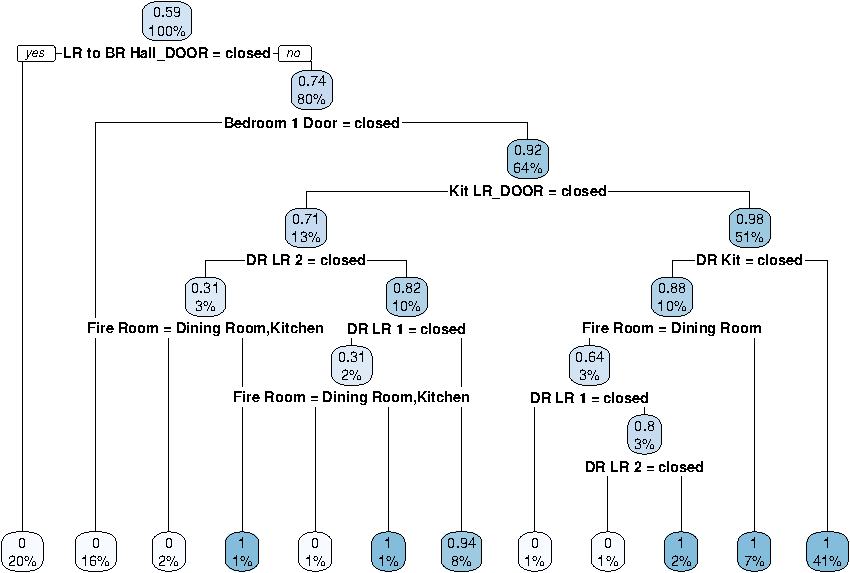
\includegraphics{ex3_files/figure-latex/cart-1.pdf}

To better understand the cases where the bedroom alarm fails to sound, a
classification tree was generated on whether the bedroom alarm sounded
(above). It is unusual for a tree to produce results as stark as this
one. What becomes clear on looking at the tree is that the state of the
intervening doors determines whether the bedroom alarm sounds. If the
fire is isolated from the bedroom by closed doors then the alarm will
not sound. Otherwise it will.

Interconnected alarms do not monitor continuously. Rather they check
periodically to see if some other alarm has sounded. For this example,
we will assume they check every 60 seconds. The effect is that there is
a random delay, with the delay drawn from a uniform random distribution
of between zero and 60 seconds. A Kernal Density estimate of the
distribution of time savings is plotted below, with fire type on
separate charts. Any negative ``time delay'' means that the bedroom
alarm sounds on its own before it gets notification from the Living Room
alarm.

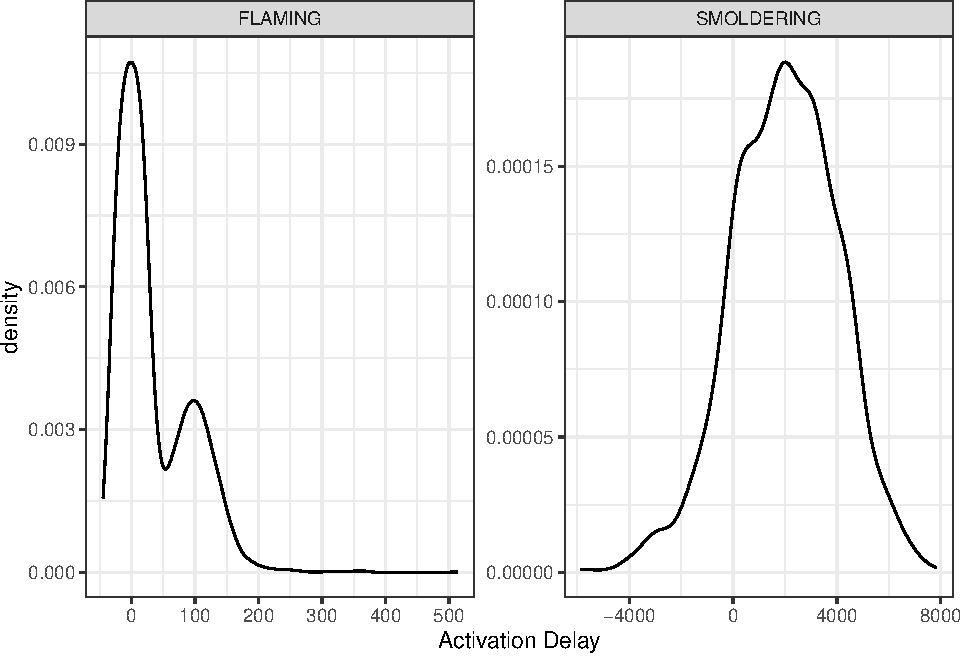
\includegraphics{ex3_files/figure-latex/kde-1.pdf}

With 10~000 data points we can empirically estimate the average time
savings that interconnected alarms would provide, as well as median time
savings and various quantiles. We are interested in the quantiles
because adverse outcomes, like death or injury, are tail events. So we
also look at the tails of the distribution. Here the ``1~\% Quantile''
means that 1~\% of alarms saved more time than this.

\begin{longtable}[]{@{}lll@{}}
\toprule
result & Flaming & Smoldering\tabularnewline
\midrule
\endhead
Mean & 101.7 & 1821.8\tabularnewline
Median & 96.0 & 1597.7\tabularnewline
25 \% Quantile & 136.3 & 2936.7\tabularnewline
10 \% Quantile & 176.4 & 4139.8\tabularnewline
5 \% Quantile & 199.5 & 4792.5\tabularnewline
1 \% Quantile & 238.3 & 6109.8\tabularnewline
\bottomrule
\end{longtable}

This looks only at cases where the Bedroom 1 alarm sounded. If this were
a serious attempt to identify the effect of interconnected alarms then
the percent of non-activations would need to be taken into account. If
non-activations were included all the quantiles larger than the median
would fall into the non-activation range.

\hypertarget{number-of-cases---revisited}{%
\subsection{Number of Cases -
Revisited}\label{number-of-cases---revisited}}

The preliminary analysis above suggested that we appeared to have enough
cases. However, the values of interest here are complex manipulations of
the data. Even though the average of the Bedroom activation time has
converged, it is possible that the results of interest to us have not.
To finally determine if we have enough cases we look at how the outcomes
we analyze change with the number of cases.

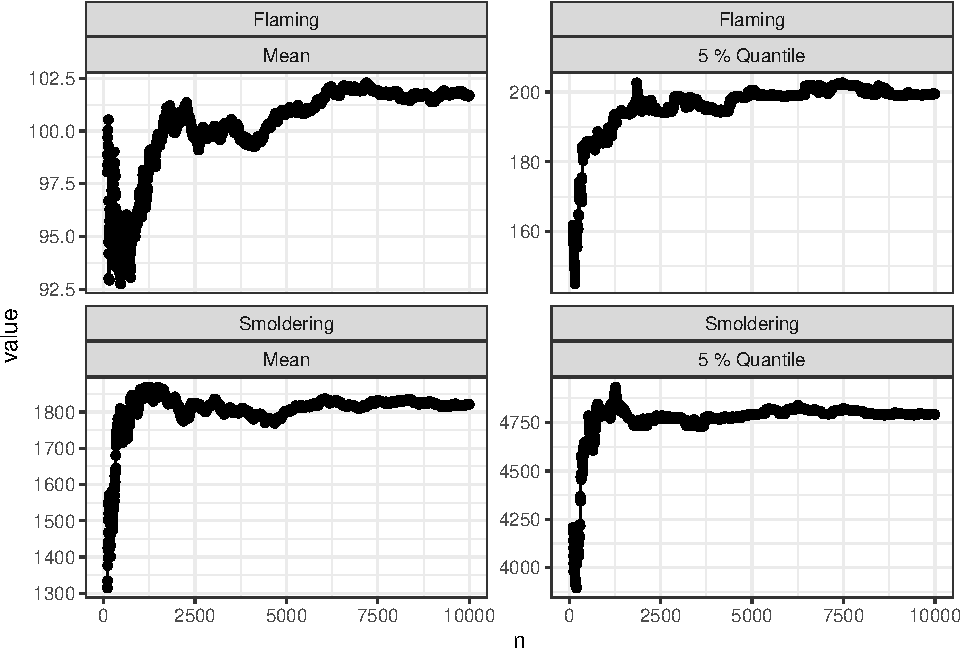
\includegraphics{ex3_files/figure-latex/cvg_plot-1.pdf}

While the preliminary look settled down within a couple of thousand
cases, these results take longer. In particular the extreme quantiles
take somewhat longer to settle down. In particular, the 5 \% quantile
value doesn't really settle down until we have 7500 cases or so.
However, looking at the results it looks like our results have settled
down sufficiently by the 10~000 cases we actually use to have reasonable
confidence in our results.

\hypertarget{discussion}{%
\subsection{Discussion}\label{discussion}}

For a study like this it is really important to get the distribution of
fire parameters correct. For example, if the proportion of fires
starting in the Kitchen were low compared to the real world then all of
the time-delay values would be underestimated. If the likelihood of
closed doors were overestimated, then there would be far fewer cases of
alarm failure for the bedroom alarms, and the benefit of interconnection
would be lower.

\begin{center}\rule{0.5\linewidth}{0.5pt}\end{center}

\hypertarget{obsolete-material}{%
\section{Obsolete Material}\label{obsolete-material}}

Here the question relates to the difference in activation times between
the closest alarm and the alarms in the bedroom area. For this example,
we will assume that there are two alarms: one in the living room (near
the kitchen but not in it), and one in bedroom 1.

There are three cases here that need to be considered for each fire
type. Cases where both alarms activate, cases where only the Living Room
alarm activates, and cases where neither alarm activates. It is
conceivable that only the bedroom alarm could activate, but such cases
do not occur in the data for the living room alarm (although they do
occur for the dining room alarm). We will drop the cases where neither
alarm activates because they are not relevant to the question being
considered.

Looking at the data, the flaming type fires clearly fall into two
groups. The ones where the bedroom alarm activate essentially all fall
into the range of 0 - 300 second difference in activation times, while
the cases where the bedroom alarm does not activate all exceed a time
difference of \textgreater{} 12000 seconds. So here, the question is:
first when does the bedroom alarm activate. Second, if the bedroom alarm
activates how big is the difference in activation times.

For the smoldering type fires, I think it is somewhat more complex.
First, I \emph{think} that there is a set of cases where time
differences are in the order of those with the flaming type fires.
Second, there are a set of cases with a mean time difference around 2500
seconds. I \emph{think} there is also a third group with a larger mean
difference as well. As with the flaming fires, there is a significant
fraction of the data where the bedroom alarm does not activate. It is
possible that this is just a censored subset of the former two
populations, but I suspect that for the most part it is a third subset
of the data.

Analysis of the flaming data set is relatively easy. First identify what
determines the difference between cases where the bedroom alarm
activates and cases where it does not. Second, characterize the data
where both alarms activate. The data is skewed (but decidedly not
log-normal). I want to see if the data can be fit to a gamma (or
similar) distribution. I also want to fit a model to the data and see
what the explanatory variables can explain.

The plot above indicates that the flaming data will fit a gamma
distribution pretty well. The dip in the KDE at the peak is a feature
not a statistical anamaly. This is a composite of the results from three
different rooms. Here the first peak is from the cases where the fire
starts in the living room, while the second peak is from the cases where
the fires starts elsewhere.

The subsequent plots compare the KDE estimate for each of the rooms of
fire origin to the best fit gamma distribution. The fits aren't bad, but
they aren't especially good either.

To the extent that I want to know the distribution of
time-differences--and that is all that I want to know--a fit to the
gamma distribution might be a good choice.

Analysis of the smoldering data will be more complicated. First, there
is the distinction between cases where the bedroom alarm activates and
cases where it does not. I think that is the first distinction to make.

Next I would try to fit a mixture distribution to the data to identify
the characteristics of the two distributions that make up the results.
As a first level estimate, I would just identify distribution parameters
to the two distributions (using the EM algorithm?). Second I would try
to fit more complex models to the two distributions (using our
covariates). Third I want to see if I can use the covariates to separate
out the two populations. I need to explore the various packages that
implement the EM algorithm and see if any will do what I want here.

\hypertarget{are-there-enough-runs}{%
\section{Are There Enough Runs?}\label{are-there-enough-runs}}

To test whether we have enough runs we look at the average result versus
number of runs (which should converge to a constant value) and the
standard devation of the mean versus number of runs, which should
converge to zero. The charts shown below are for the Bedroom 3 alarm
time. There are four charts per figure. The ``flaming'' charts are for
flaming ignitions while the ``smoldering'' charts are for smoldering
ignitions. The ``alert'' charts represent the proportion of runs in
which the alarm sounded within the time of the simulation, while the
``times'' models are for the time to sound conditional on the alarm
sounding within the time of the simulation.

\hypertarget{discussion-1}{%
\section{Discussion}\label{discussion-1}}

\end{document}
